\hypertarget{sec-preprocessing}{%
\chapter{Preprocessing}\label{sec-preprocessing}}

\vspace{-15mm}\addtocontents{toc}{\textit{Janek Thomas}}

\textbf{Janek Thomas} \newline  \emph{Ludwig-Maximilians-Universität
München, and Munich Center for Machine Learning (MCML), and Essential
Data Science Training GmbH} \newline \newline 

Chapter~\ref{sec-pipelines} and Chapter~\ref{sec-pipelines-nonseq}
provided a technical introduction to
\href{https://mlr3pipelines.mlr-org.com}{\texttt{mlr3pipelines}}\index{\texttt{mlr3pipelines}},
this chapter will now demonstrate how to use those pipelines to tackle
common problems when preprocessing\index{preprocessing} data for ML,
including factor encoding\index{factor encoding},
imputation\index{imputation} of missing values, feature and target
transformations, and functional feature
extraction\index{feature extraction}. Feature selection, an important
preprocessing method, is covered in Chapter~\ref{sec-feature-selection}.

In this book, preprocessing refers to everything that happens with
\emph{data} before it is used to fit a model, while
postprocessing\index{postprocessing} encompasses everything that occurs
with \emph{predictions} after the model is fitted.

Data cleaning\index{data cleaning}{\marginnote{\begin{footnotesize}Data
Cleaning\end{footnotesize}}}\index{exploratory data analysis|see{data cleaning}}
is an important part of preprocessing that involves the removal of
errors, noise, and redundancy in the data; we only consider data
cleaning very briefly as it is usually performed outside of
\texttt{mlr3} on the raw dataset.

Another aspect of preprocessing is feature
engineering\index{feature engineering}{\marginnote{\begin{footnotesize}Feature
Engineering\end{footnotesize}}}, which covers all other transformations
of data before it is fed to the machine learning model, including the
creation of features from possibly unstructured data, such as written
text, sequences or images. The goal of feature engineering is to enable
the data to be handled by a given learner, and/or to further improve
predictive performance. It is important to note that feature engineering
helps mostly for simpler algorithms, while highly complex models usually
gain less from it and require little data preparation to be trained.
Common difficulties in data that can be solved with feature engineering
include features with skewed distributions, high cardinality categorical
features, missing observations, high dimensionality and imbalanced
classes in classification tasks. Deep learning has shown promising
results in automating feature engineering, however, its effectiveness
depends on the complexity and nature of the data being processed, as
well as the specific problem being addressed. Typically it can work well
with natural language processing and computer vision problems, while for
standard tabular data, tree-based ensembles such as a random forest or
gradient boosting are often still superior (and easier to handle).
However, tabular deep learning approaches are currently catching up
quickly. Hence, manual feature engineering is still often required but
with \texttt{mlr3pipelines}, which can simplify the process as much as
possible.

As we work through this chapter we will use an adapted version of the
Ames housing data (De Cock 2011). We changed the data slightly and
introduced some additional (artificial) problems to showcase as many
aspects of preprocessing as possible on a single dataset. The modified
version is shipped with
\href{https://mlr3data.mlr-org.com}{\texttt{mlr3data}} and the code to
recreate this version of the data from the original raw data can be
found at \url{https://github.com/mlr-org/mlr3data/} in the directory
\texttt{data-raw}. This original dataset was collected as an alternative
to the Boston Housing data and is commonly used to demonstrate feature
engineering in ML. Raw and processed versions of the data can be
directly loaded from the
\href{https://cran.r-project.org/package=AmesHousing}{\texttt{AmesHousing}}
package. The dataset includes 2,930 residential properties (rows)
situated in Ames, Iowa, sold between 2006 and 2010. It contains 81
features about various aspects of the property, the size and shape of
the lot, and information about its condition and quality. The prediction
target is the sale price in USD, hence it is a regression task.

\begin{Shaded}
\begin{Highlighting}[]
\NormalTok{ames }\OtherTok{=}\NormalTok{ mlr3data}\SpecialCharTok{::}\NormalTok{ames\_housing}
\end{Highlighting}
\end{Shaded}

\hypertarget{data-cleaning}{%
\section{Data Cleaning}\label{data-cleaning}}

As a first step, we explore the data and look for simple problems such
as constant or duplicated features. This can be done quite efficiently
with a package like
\href{https://cran.r-project.org/package=DataExplorer}{\texttt{DataExplorer}}
or \href{https://cran.r-project.org/package=skimr}{\texttt{skimr}} which
can be used to create a large number of informative plots.

Below we summarize the most important findings for data cleaning, but we
only consider this aspect in a cursory manner:

\begin{Shaded}
\begin{Highlighting}[]
\CommentTok{\# 1. \textasciigrave{}Misc\_Feature\_2\textasciigrave{} is a factor with only a single level \textasciigrave{}Othr\textasciigrave{}.}
\FunctionTok{summary}\NormalTok{(ames}\SpecialCharTok{$}\NormalTok{Misc\_Feature\_2)}
\end{Highlighting}
\end{Shaded}

\begin{verbatim}
Othr 
2930 
\end{verbatim}

\begin{Shaded}
\begin{Highlighting}[]
\CommentTok{\# 2. \textasciigrave{}Condition\_2\textasciigrave{} and \textasciigrave{}Condition\_3\textasciigrave{} are identical.}
\FunctionTok{identical}\NormalTok{(ames}\SpecialCharTok{$}\NormalTok{Condition\_2, ames}\SpecialCharTok{$}\NormalTok{Condition\_3)}
\end{Highlighting}
\end{Shaded}

\begin{verbatim}
[1] TRUE
\end{verbatim}

\begin{Shaded}
\begin{Highlighting}[]
\CommentTok{\# 3. \textasciigrave{}Lot\_Area\textasciigrave{} and \textasciigrave{}Lot\_Area\_m2\textasciigrave{} are same data on different scales}
\FunctionTok{cor}\NormalTok{(ames}\SpecialCharTok{$}\NormalTok{Lot\_Area, ames}\SpecialCharTok{$}\NormalTok{Lot\_Area\_m2)}
\end{Highlighting}
\end{Shaded}

\begin{verbatim}
[1] 1
\end{verbatim}

For all three problems, simply removing the problematic features (or
feature in a pair) might be the best course of action.

\begin{Shaded}
\begin{Highlighting}[]
\NormalTok{to\_remove }\OtherTok{=} \FunctionTok{c}\NormalTok{(}\StringTok{"Lot\_Area\_m2"}\NormalTok{, }\StringTok{"Condition\_3"}\NormalTok{, }\StringTok{"Misc\_Feature\_2"}\NormalTok{)}
\end{Highlighting}
\end{Shaded}

Other typical problems that should be checked are:

\begin{enumerate}
\def\labelenumi{\arabic{enumi}.}
\tightlist
\item
  ID columns, i.e., columns that are unique for every observation should
  be removed or tagged.
\item
  \texttt{NA}s not correctly encoded, e.g.~as \texttt{"NA"} or
  \texttt{""}
\item
  Semantic errors in the data, e.g., negative \texttt{Lot\_Area}
\item
  Numeric features encoded as categorical for learners that can not
  handle such features.
\end{enumerate}

Before we continue with feature engineering we will create a task,
measure, and resampling strategy to use throughout the chapter.

\begin{Shaded}
\begin{Highlighting}[]
\NormalTok{tsk\_ames }\OtherTok{=} \FunctionTok{as\_task\_regr}\NormalTok{(ames, }\AttributeTok{target =} \StringTok{"Sale\_Price"}\NormalTok{, }\AttributeTok{id =} \StringTok{"ames"}\NormalTok{)}
\CommentTok{\# remove problematic features}
\NormalTok{tsk\_ames}\SpecialCharTok{$}\FunctionTok{select}\NormalTok{(}\FunctionTok{setdiff}\NormalTok{(tsk\_ames}\SpecialCharTok{$}\NormalTok{feature\_names, to\_remove))}

\NormalTok{msr\_mae }\OtherTok{=} \FunctionTok{msr}\NormalTok{(}\StringTok{"regr.mae"}\NormalTok{)}
\NormalTok{rsmp\_cv3 }\OtherTok{=} \FunctionTok{rsmp}\NormalTok{(}\StringTok{"cv"}\NormalTok{, }\AttributeTok{folds =} \DecValTok{3}\NormalTok{)}
\NormalTok{rsmp\_cv3}\SpecialCharTok{$}\FunctionTok{instantiate}\NormalTok{(tsk\_ames)}
\end{Highlighting}
\end{Shaded}

Lastly, we run a very simple experiment to verify our setup works as
expected with a simple featureless baseline, note below we set
\texttt{robust\ =\ TRUE} to always predict the \emph{median} sale price
as opposed to the \emph{mean}.

\begin{Shaded}
\begin{Highlighting}[]
\NormalTok{lrn\_baseline }\OtherTok{=} \FunctionTok{lrn}\NormalTok{(}\StringTok{"regr.featureless"}\NormalTok{, }\AttributeTok{robust =} \ConstantTok{TRUE}\NormalTok{)}
\NormalTok{lrn\_baseline}\SpecialCharTok{$}\NormalTok{id }\OtherTok{=} \StringTok{"Baseline"}
\NormalTok{rr\_baseline }\OtherTok{=} \FunctionTok{resample}\NormalTok{(tsk\_ames, lrn\_baseline, rsmp\_cv3)}
\NormalTok{rr\_baseline}\SpecialCharTok{$}\FunctionTok{aggregate}\NormalTok{(msr\_mae)}
\end{Highlighting}
\end{Shaded}

\begin{verbatim}
regr.mae 
   56056 
\end{verbatim}

\hypertarget{factor-encoding}{%
\section{Factor Encoding}\label{factor-encoding}}

Many machine learning algorithm implementations, such as XGBoost (Chen
and Guestrin 2016), cannot handle categorical data and so categorical
features must be encoded\index{encoding} into numerical variables.

\begin{Shaded}
\begin{Highlighting}[]
\NormalTok{lrn\_xgb }\OtherTok{=} \FunctionTok{lrn}\NormalTok{(}\StringTok{"regr.xgboost"}\NormalTok{, }\AttributeTok{nrounds =} \DecValTok{100}\NormalTok{)}
\NormalTok{lrn\_xgb}\SpecialCharTok{$}\FunctionTok{train}\NormalTok{(tsk\_ames)}
\end{Highlighting}
\end{Shaded}

\begin{verbatim}
Error: <TaskRegr:ames> has the following unsupported feature types: factor
\end{verbatim}

Categorical features can be grouped by their cardinality, which refers
to the number of levels they contain: binary features (two levels),
low-cardinality features, and high-cardinality features; there is no
universal threshold for when a feature should be considered
high-cardinality and this threshold can even be tuned. For now, we will
consider high-cardinality to be features with more than 10 levels:

\begin{Shaded}
\begin{Highlighting}[]
\FunctionTok{names}\NormalTok{(}\FunctionTok{which}\NormalTok{(}\FunctionTok{lengths}\NormalTok{(tsk\_ames}\SpecialCharTok{$}\FunctionTok{levels}\NormalTok{()) }\SpecialCharTok{\textgreater{}} \DecValTok{10}\NormalTok{))}
\end{Highlighting}
\end{Shaded}

\begin{verbatim}
[1] "Exterior_1st" "Exterior_2nd" "MS_SubClass"  "Neighborhood"
\end{verbatim}

Binary features can be trivially encoded by setting one of the feature
levels to \texttt{1} and the other to \texttt{0}.

\begin{Shaded}
\begin{Highlighting}[]
\FunctionTok{names}\NormalTok{(}\FunctionTok{which}\NormalTok{(}\FunctionTok{lengths}\NormalTok{(tsk\_ames}\SpecialCharTok{$}\FunctionTok{levels}\NormalTok{()) }\SpecialCharTok{==} \DecValTok{2}\NormalTok{))}
\end{Highlighting}
\end{Shaded}

\begin{verbatim}
[1] "Alley"       "Central_Air" "Street"     
\end{verbatim}

Low-cardinality features can be handled by one-hot
encoding\index{encoding!one-hot}{\marginnote{\begin{footnotesize}One-hot
Encoding\end{footnotesize}}}. One-hot encoding is a process of
converting categorical features into a binary representation, where each
possible category is represented as a separate binary feature.
Theoretically, it is sufficient to create one less binary feature than
levels, as setting all binary features to zero is also a valid
representation. This is typically called
dummy\index{dummy encoding|see{encoding, treatment}} or treatment
encoding\index{encoding!treatment} and is required if the learner is a
generalized linear model (GLM) or additive model
(GAM)\index{generalized linear model}.

Some learners support handling categorical features but may still crash
for high-cardinality features if they internally apply encodings that
are only suitable for low-cardinality features, such as one-hot
encoding. Impact encoding (Micci-Barreca 2001) is a good approach for
handling high-cardinality features. Impact
encoding\index{encoding!impact}{\marginnote{\begin{footnotesize}Impact
Encoding\end{footnotesize}}} converts categorical features into numeric
values. The idea behind impact encoding is to use the target feature to
create a mapping between the categorical feature and a numerical value
that reflects its importance in predicting the target feature. Impact
encoding involves the following steps:

\begin{enumerate}
\def\labelenumi{\arabic{enumi}.}
\tightlist
\item
  Group the target variable by the categorical feature.
\item
  Compute the mean of the target variable for each group.
\item
  Compute the global mean of the target variable.
\item
  Compute the impact score for each group as the difference between the
  mean of the target variable for the group and the global mean of the
  target variable.
\item
  Replace the categorical feature with the impact scores.
\end{enumerate}

Impact encoding preserves the information of the categorical feature
while also creating a numerical representation that reflects its
importance in predicting the target. Compared to one-hot encoding, the
main advantage is that only a single numeric feature is created
regardless of the number of levels of the categorical features, hence it
is especially useful for high-cardinality features. As information from
the target is used to compute the impact scores, the encoding process
must be embedded in cross-validation to avoid leakage between training
and testing data (Chapter~\ref{sec-performance}).

As well as encoding features, other basic preprocessing steps for
categorical features include removing constant features (which only have
one level and may have been removed as part of data cleaning), and
collapsing levels that occur very rarely. These types of problems can
occur as artifacts of resampling as the dataset size is further reduced.
Stratification on such features would be an alternative way to mitigate
this (Section~\ref{sec-strat-group}).

In the code below we use \texttt{po("removeconstants")} to remove
features with only one level, \texttt{po("collapsefactors")} to collapse
levels that occur less than 1\% of the time in the data,
\texttt{po("encodeimpact")} to impact-encode high-cardinality features,
\texttt{po("encode",\ method\ =\ "one-hot")} to one-hot encode
low-cardinality features, and finally
\texttt{po("encode",\ method\ =\ "treatment")} to treatment encode
binary features.

\begin{Shaded}
\begin{Highlighting}[]
\NormalTok{factor\_pipeline }\OtherTok{=}
    \FunctionTok{po}\NormalTok{(}\StringTok{"removeconstants"}\NormalTok{) }\SpecialCharTok{\%\textgreater{}\textgreater{}\%}
    \FunctionTok{po}\NormalTok{(}\StringTok{"collapsefactors"}\NormalTok{, }\AttributeTok{no\_collapse\_above\_prevalence =} \FloatTok{0.01}\NormalTok{) }\SpecialCharTok{\%\textgreater{}\textgreater{}\%}
    \FunctionTok{po}\NormalTok{(}\StringTok{"encodeimpact"}\NormalTok{,}
        \AttributeTok{affect\_columns =} \FunctionTok{selector\_cardinality\_greater\_than}\NormalTok{(}\DecValTok{10}\NormalTok{),}
        \AttributeTok{id =} \StringTok{"high\_card\_enc"}\NormalTok{) }\SpecialCharTok{\%\textgreater{}\textgreater{}\%}
    \FunctionTok{po}\NormalTok{(}\StringTok{"encode"}\NormalTok{, }\AttributeTok{method =} \StringTok{"one{-}hot"}\NormalTok{,}
        \AttributeTok{affect\_columns =} \FunctionTok{selector\_cardinality\_greater\_than}\NormalTok{(}\DecValTok{2}\NormalTok{),}
        \AttributeTok{id =} \StringTok{"low\_card\_enc"}\NormalTok{) }\SpecialCharTok{\%\textgreater{}\textgreater{}\%}
    \FunctionTok{po}\NormalTok{(}\StringTok{"encode"}\NormalTok{, }\AttributeTok{method =} \StringTok{"treatment"}\NormalTok{,}
        \AttributeTok{affect\_columns =} \FunctionTok{selector\_type}\NormalTok{(}\StringTok{"factor"}\NormalTok{), }\AttributeTok{id =} \StringTok{"binary\_enc"}\NormalTok{)}
\end{Highlighting}
\end{Shaded}

Now we can apply this pipeline to our xgboost model to use it in a
benchmark experiment; we also compare a simpler pipeline that only uses
one-hot encoding to demonstrate performance differences resulting from
different strategies.

\begin{Shaded}
\begin{Highlighting}[]
\NormalTok{glrn\_xgb\_impact }\OtherTok{=} \FunctionTok{as\_learner}\NormalTok{(factor\_pipeline }\SpecialCharTok{\%\textgreater{}\textgreater{}\%}\NormalTok{ lrn\_xgb)}
\NormalTok{glrn\_xgb\_impact}\SpecialCharTok{$}\NormalTok{id }\OtherTok{=} \StringTok{"XGB\_enc\_impact"}

\NormalTok{glrn\_xgb\_one\_hot }\OtherTok{=} \FunctionTok{as\_learner}\NormalTok{(}\FunctionTok{po}\NormalTok{(}\StringTok{"encode"}\NormalTok{) }\SpecialCharTok{\%\textgreater{}\textgreater{}\%}\NormalTok{ lrn\_xgb)}
\NormalTok{glrn\_xgb\_one\_hot}\SpecialCharTok{$}\NormalTok{id }\OtherTok{=} \StringTok{"XGB\_enc\_onehot"}

\NormalTok{bmr }\OtherTok{=} \FunctionTok{benchmark}\NormalTok{(}\FunctionTok{benchmark\_grid}\NormalTok{(tsk\_ames,}
  \FunctionTok{c}\NormalTok{(lrn\_baseline, glrn\_xgb\_impact, glrn\_xgb\_one\_hot), rsmp\_cv3))}
\NormalTok{bmr}\SpecialCharTok{$}\FunctionTok{aggregate}\NormalTok{(}\AttributeTok{measure =}\NormalTok{ msr\_mae)[, .(learner\_id, regr.mae)]}
\end{Highlighting}
\end{Shaded}

\begin{verbatim}
       learner_id regr.mae
1:       Baseline    56056
2: XGB_enc_impact    16068
3: XGB_enc_onehot    16098
\end{verbatim}

In this small experiment, we see that the difference between the
extended factor encoding pipeline and the simpler one-hot encoding
strategy pipeline is only very small. If you are interested in learning
more about different encoding strategies, including a benchmark study
comparing them, we recommend Pargent et al. (2022).

\hypertarget{sec-preprocessing-missing}{%
\section{Missing Values}\label{sec-preprocessing-missing}}

A common problem in real-world data is missing
values\index{missing data} in features. In the Ames dataset, several
variables have at least one missing data point:

\begin{Shaded}
\begin{Highlighting}[]
\CommentTok{\# print first five with missing data}
\FunctionTok{names}\NormalTok{(}\FunctionTok{which}\NormalTok{(tsk\_ames}\SpecialCharTok{$}\FunctionTok{missings}\NormalTok{() }\SpecialCharTok{\textgreater{}} \DecValTok{0}\NormalTok{))[}\DecValTok{1}\SpecialCharTok{:}\DecValTok{5}\NormalTok{]}
\end{Highlighting}
\end{Shaded}

\begin{verbatim}
[1] "Alley"          "BsmtFin_SF_1"   "BsmtFin_SF_2"   "BsmtFin_Type_1"
[5] "BsmtFin_Type_2"
\end{verbatim}

Many learners cannot handle missing values automatically (e.g.,
\texttt{lrn("regr.ranger")} and \texttt{lrn("regr.lm")}) and others may
be able to handle missing values but may use simple methods that are not
ideal (e.g., just omitting rows with missing data).

The simplest data
imputation\index{data imputation}{\marginnote{\begin{footnotesize}Data
Imputation\end{footnotesize}}} method is to replace missing values by
the feature's mean (\texttt{po("imputemean")})
(Figure~\ref{fig-imputation}), median (\texttt{po("imputemedian")}), or
mode (\texttt{po("imputemode")}). Alternatively, one can impute by
sampling from the empirical distribution of the feature, for example a
histogram (\texttt{po("imputehist")}). Instead of guessing at what a
missing feature might be, missing values could instead be replaced by a
new level, for example, called \texttt{.MISSING}
(\texttt{po("imputeoor")}). For numeric features, Ding and Simonoff
(2010) show that for binary classification and tree-based models,
encoding missing values out-of-range (OOR), e.g.~a constant value above
the largest observed value, is a reasonable approach.

\begin{figure}

{\centering 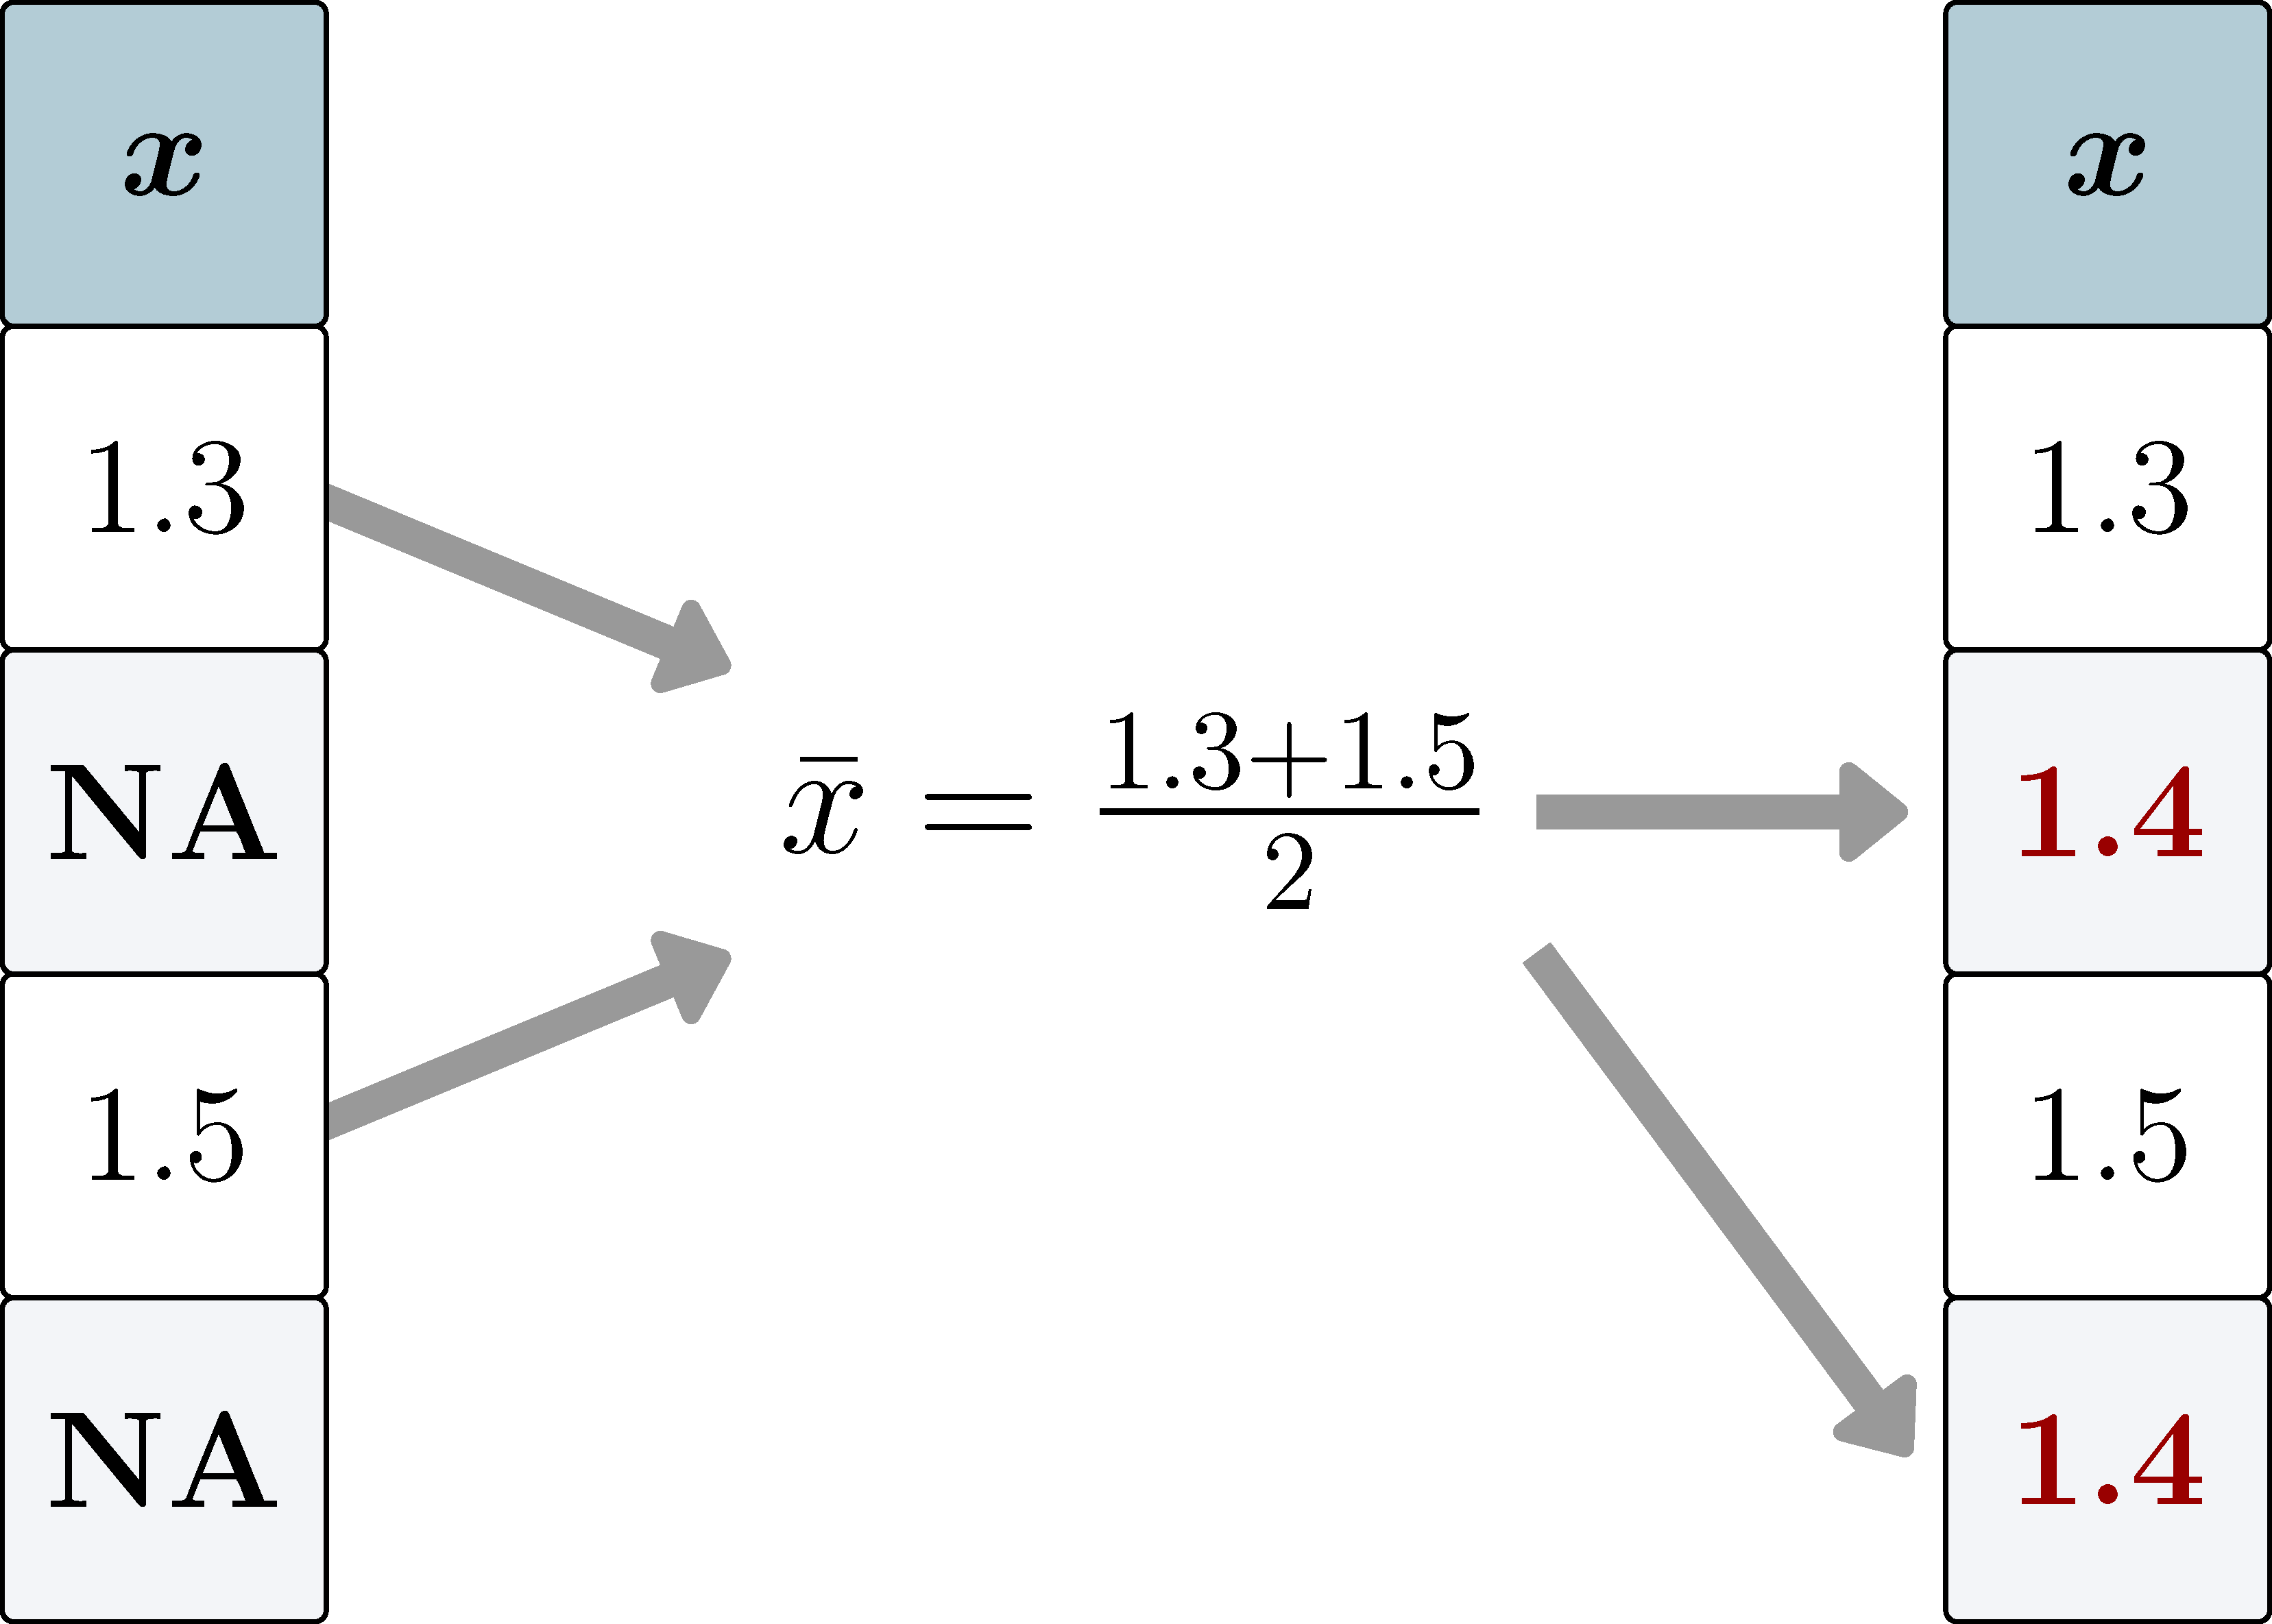
\includegraphics[width=0.6\textwidth,height=\textheight]{chapters/chapter9/Figures/mlr3book_figures-13.png}

}

\caption{\label{fig-imputation}Mean imputation of missing values using
observed values.}

\end{figure}

It is often important for predictive tasks that you keep track of
missing data as it is common for missing data to be informative in
itself. To preserve the information about which data was missing,
imputation should be tracked by adding binary indicator features (one
for each imputed feature) that are \texttt{1} if the feature was missing
for an observation and \texttt{0} if it was present
(\texttt{po("missind")}). It is important to note that recording this
information will not prevent problems in model interpretation on its
own. As a real-world example, medical data are typically collected more
extensively for White communities than for racially minoritized
communities. Imputing data from minoritized communities would at best
mask this data bias, and at worst would make the data bias even worse by
making vastly inaccurate assumptions (see Chapter~\ref{sec-fairness} for
data bias and algorithmic fairness).

In the code below we create a pipeline from the
\href{https://mlr3pipelines.mlr-org.com/reference/PipeOp.html}{\texttt{PipeOp}}s
listed above as well as making use of \texttt{po("featureunion")} to
combine multiple \texttt{PipeOp}s acting on the \texttt{"integer"}
columns.

\begin{Shaded}
\begin{Highlighting}[]
\NormalTok{impute\_hist }\OtherTok{=} \FunctionTok{list}\NormalTok{(}
      \FunctionTok{po}\NormalTok{(}\StringTok{"missind"}\NormalTok{, }\AttributeTok{type =} \StringTok{"integer"}\NormalTok{,}
          \AttributeTok{affect\_columns =} \FunctionTok{selector\_type}\NormalTok{(}\StringTok{"integer"}\NormalTok{)}
\NormalTok{      ),}
      \FunctionTok{po}\NormalTok{(}\StringTok{"imputehist"}\NormalTok{, }\AttributeTok{affect\_columns =} \FunctionTok{selector\_type}\NormalTok{(}\StringTok{"integer"}\NormalTok{))}
\NormalTok{    ) }\SpecialCharTok{\%\textgreater{}\textgreater{}\%}
    \FunctionTok{po}\NormalTok{(}\StringTok{"featureunion"}\NormalTok{) }\SpecialCharTok{\%\textgreater{}\textgreater{}\%}
    \FunctionTok{po}\NormalTok{(}\StringTok{"imputeoor"}\NormalTok{, }\AttributeTok{affect\_columns =} \FunctionTok{selector\_type}\NormalTok{(}\StringTok{"factor"}\NormalTok{))}

\NormalTok{impute\_hist}\SpecialCharTok{$}\FunctionTok{plot}\NormalTok{(}\AttributeTok{horizontal =} \ConstantTok{TRUE}\NormalTok{)}
\end{Highlighting}
\end{Shaded}

\begin{figure}

{\centering 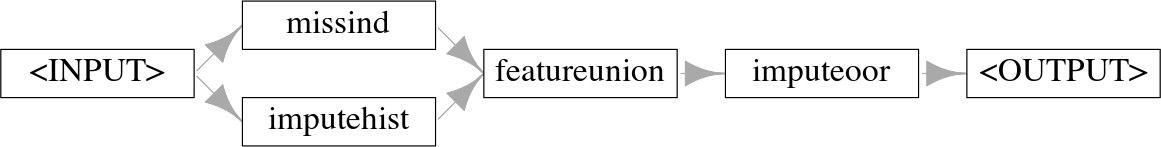
\includegraphics[width=1\textwidth,height=\textheight]{chapters/chapter9/preprocessing_files/figure-pdf/fig-impute-1.png}

}

\caption{\label{fig-impute}Pipeline to impute missing values of numeric
features by histogram with binary indicators and missings in
categoricals out-of-range with a new level.}

\end{figure}

Using this pipeline we can now run experiments with
\texttt{lrn("regr.ranger")}, which cannot handle missing data; we also
compare a simpler pipeline that only uses OOR imputation to demonstrate
performance differences resulting from different strategies.

\begin{Shaded}
\begin{Highlighting}[]
\NormalTok{glrn\_rf\_impute\_hist }\OtherTok{=} \FunctionTok{as\_learner}\NormalTok{(impute\_hist }\SpecialCharTok{\%\textgreater{}\textgreater{}\%} \FunctionTok{lrn}\NormalTok{(}\StringTok{"regr.ranger"}\NormalTok{))}
\NormalTok{glrn\_rf\_impute\_hist}\SpecialCharTok{$}\NormalTok{id }\OtherTok{=} \StringTok{"RF\_imp\_Hist"}

\NormalTok{glrn\_rf\_impute\_oor }\OtherTok{=} \FunctionTok{as\_learner}\NormalTok{(}\FunctionTok{po}\NormalTok{(}\StringTok{"imputeoor"}\NormalTok{) }\SpecialCharTok{\%\textgreater{}\textgreater{}\%} \FunctionTok{lrn}\NormalTok{(}\StringTok{"regr.ranger"}\NormalTok{))}
\NormalTok{glrn\_rf\_impute\_oor}\SpecialCharTok{$}\NormalTok{id }\OtherTok{=} \StringTok{"RF\_imp\_OOR"}

\NormalTok{design }\OtherTok{=} \FunctionTok{benchmark\_grid}\NormalTok{(tsk\_ames,}
  \FunctionTok{c}\NormalTok{(glrn\_rf\_impute\_hist, glrn\_rf\_impute\_oor), rsmp\_cv3)}
\NormalTok{bmr\_new }\OtherTok{=} \FunctionTok{benchmark}\NormalTok{(design)}
\NormalTok{bmr}\SpecialCharTok{$}\FunctionTok{combine}\NormalTok{(bmr\_new)}
\NormalTok{bmr}\SpecialCharTok{$}\FunctionTok{aggregate}\NormalTok{(}\AttributeTok{measure =}\NormalTok{ msr\_mae)[, .(learner\_id, regr.mae)]}
\end{Highlighting}
\end{Shaded}

\begin{verbatim}
       learner_id regr.mae
1:       Baseline    56056
2: XGB_enc_impact    16068
3: XGB_enc_onehot    16098
4:    RF_imp_Hist    16377
5:     RF_imp_OOR    16393
\end{verbatim}

Similarly to encoding, we see limited differences in performance between
the different imputation strategies. This is expected here and confirms
the findings of Ding and Simonoff (2010) -- out-of-range imputation is a
simple yet effective imputation for tree-based methods.

Many more advanced imputation strategies exist, including model-based
imputation where machine learning models are used to predict missing
values, and multiple imputation where data is repeatedly resampled and
imputed in each sample (e.g., by mean imputation) to attain more robust
estimates. However, these more advanced techniques rarely improve the
models predictive performance substantially and the simple imputation
techniques introduced above are usually sufficient (Poulos and Valle
2018). Nevertheless, these methods are still important, as finding
imputations that fit well to the distribution of the observed values
allows a model to be fitted that can be interpreted and analyzed in a
second step.

\hypertarget{sec-prepro-robustify}{%
\section{Pipeline Robustify}\label{sec-prepro-robustify}}

\texttt{mlr3pipelines} offers a simple and reusable pipeline for (among
other things) imputation\index{imputation} and factor
encoding\index{encoding} called
\texttt{ppl("robustify")}\index{\texttt{ppl("robustify")}}{\marginnote{\begin{footnotesize}ppl(``robustify'')\end{footnotesize}}},
which includes sensible defaults that can be used most of the time when
encoding or imputing data. The pipeline includes the following
\href{https://mlr3pipelines.mlr-org.com/reference/PipeOp.html}{\texttt{PipeOp}}s
(some are applied multiple times and most use selectors):

\begin{enumerate}
\def\labelenumi{\arabic{enumi}.}
\tightlist
\item
  \texttt{po("removeconstants")} -- Constant features are removed.
\item
  \texttt{po("colapply")} -- Character and ordinal features are encoded
  as categorical, and date/time features are encoded as numeric.
\item
  \texttt{po("imputehist")} -- Numeric features are imputed by histogram
  sampling.
\item
  \texttt{po("imputesample")} -- Logical features are imputed by
  sampling from the empirical distribution -- this only affects the
  \texttt{\$predict()}-step.
\item
  \texttt{po("missind")} -- Missing data indicators are added for
  imputed numeric and logical variables.
\item
  \texttt{po("imputeoor")} -- Missing values of categorical features are
  encoded with a new level.
\item
  \texttt{po("fixfactors")} -- Fixes levels of categorical features such
  that the same levels are present during prediction and training (which
  may involve dropping empty factor levels).
\item
  \texttt{po("imputesample")} -- Missing values in categorical features
  introduced from dropping levels in the previous step are imputed by
  sampling from the empirical distributions.
\item
  \texttt{po("collapsefactors")} -- Categorical features levels are
  collapsed (starting from the rarest factors in the training data)
  until there are less than a certan number of levels, controlled by the
  \texttt{max\_cardinality} argument (with a conservative default of
  \texttt{1000}).
\item
  \texttt{po("encode")} -- Categorical features are one-hot encoded.
\item
  \texttt{po("removeconstants")} -- Constant features that might have
  been created in the previous steps are removed.
\end{enumerate}

\texttt{ppl("robustify")} has optional arguments \texttt{task} and
\texttt{learner}. If these are provided, then the resulting pipeline
will be set up to handle the given task and learner specifically, for
example, it will not impute missing values if the learner has the
\texttt{"missings"} property, or if there are no missing values in the
task to begin with. By default, when \texttt{task} and \texttt{learner}
are not provided, the graph is set up to be defensive: it imputes all
missing values and converts all feature types to numerics.

Linear regression is a simple model that cannot handle most problems
that we may face when processing data, but with the
\texttt{ppl("robustify")} we can now include it in our experiment:

\begin{Shaded}
\begin{Highlighting}[]
\NormalTok{glrn\_lm\_robust }\OtherTok{=} \FunctionTok{as\_learner}\NormalTok{(}\FunctionTok{ppl}\NormalTok{(}\StringTok{"robustify"}\NormalTok{) }\SpecialCharTok{\%\textgreater{}\textgreater{}\%} \FunctionTok{lrn}\NormalTok{(}\StringTok{"regr.lm"}\NormalTok{))}
\NormalTok{glrn\_lm\_robust}\SpecialCharTok{$}\NormalTok{id }\OtherTok{=} \StringTok{"lm\_robust"}

\NormalTok{bmr\_new }\OtherTok{=} \FunctionTok{benchmark}\NormalTok{(}\FunctionTok{benchmark\_grid}\NormalTok{(tsk\_ames, glrn\_lm\_robust,  rsmp\_cv3))}
\NormalTok{bmr}\SpecialCharTok{$}\FunctionTok{combine}\NormalTok{(bmr\_new)}
\NormalTok{bmr}\SpecialCharTok{$}\FunctionTok{aggregate}\NormalTok{(}\AttributeTok{measure =}\NormalTok{ msr\_mae)[, .(learner\_id, regr.mae)]}
\end{Highlighting}
\end{Shaded}

\begin{verbatim}
       learner_id regr.mae
1:       Baseline    56056
2: XGB_enc_impact    16068
3: XGB_enc_onehot    16098
4:    RF_imp_Hist    16377
5:     RF_imp_OOR    16393
6:      lm_robust    16298
\end{verbatim}

Robustifying the linear regression results in a model that vastly
outperforms the featureless baseline and is competitive when compared to
more complex machine learning models.

\hypertarget{sec-prepro-scale}{%
\section{Transforming Features and Targets}\label{sec-prepro-scale}}

Simple transformations of features and the target can be beneficial (and
sometimes essential) for certain learners. In particular, log
transformation of the target can help in making the distribution more
symmetrical and can help reduce the impact of outliers. Similarly, log
transformation of skewed features can help to reduce the influence of
outliers. In Figure~\ref{fig-sale} we plot the distribution of the
target in the \texttt{ames} dataset and then the log-transformed target,
we can see how simply taking the log of the variable results in a
distribution that is much more symmetrical and with fewer outliers.

\begin{Shaded}
\begin{Highlighting}[]
\FunctionTok{library}\NormalTok{(patchwork)}

\CommentTok{\# copy ames data}
\NormalTok{log\_ames }\OtherTok{=} \FunctionTok{copy}\NormalTok{(ames)}
\CommentTok{\# log transform target}
\NormalTok{log\_ames[, logSalePrice }\SpecialCharTok{:}\ErrorTok{=} \FunctionTok{log}\NormalTok{(Sale\_Price)]}
\CommentTok{\# plot}
\FunctionTok{autoplot}\NormalTok{(}\FunctionTok{as\_task\_regr}\NormalTok{(log\_ames, }\AttributeTok{target =} \StringTok{"Sale\_Price"}\NormalTok{)) }\SpecialCharTok{+}
  \FunctionTok{autoplot}\NormalTok{(}\FunctionTok{as\_task\_regr}\NormalTok{(log\_ames, }\AttributeTok{target =} \StringTok{"logSalePrice"}\NormalTok{))}
\end{Highlighting}
\end{Shaded}

\begin{figure}

{\centering 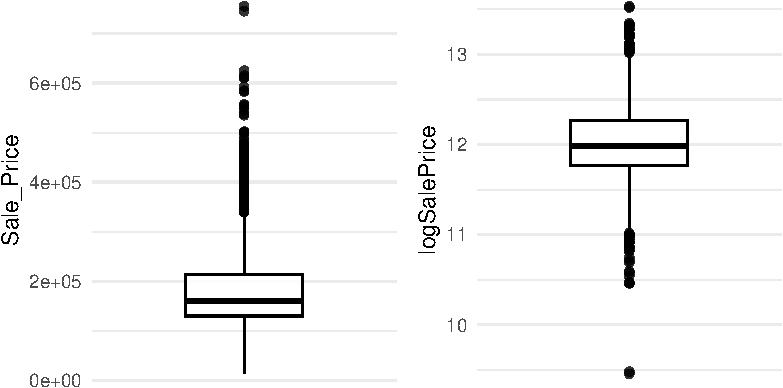
\includegraphics[width=1\textwidth,height=\textheight]{chapters/chapter9/preprocessing_files/figure-pdf/fig-sale-1.pdf}

}

\caption{\label{fig-sale}Distribution of house sales prices (in USD) in
the ames dataset before (left) and after (right) log transformation.
Before transformation there is a skewed distribution of prices towards
cheaper properties with a few outliers of very expensive properties.
After transformation the distribution is much more symmetrical with the
majority of points evenly spread around the same range.}

\end{figure}

Normalization of features may also be necessary to ensure features with
a larger scale do not have a higher impact, which is especially
important for distance-based methods such as k-nearest
neighbors\index{k-nearest neighbors} models or regularized parametric
models such as Lasso or Elastic net. Many models internally scale the
data if required by the algorithm so most of the time we do not need to
manually do this in preprocessing, though if this is required then
\texttt{po("scale")} can be used to center and scale numeric features.

Any transformations applied to the target during training must be
inverted during model prediction to ensure predictions are made on the
correct scale. By example, say we are interested in log transforming the
target, then we would take the following steps:

\begin{Shaded}
\begin{Highlighting}[]
\NormalTok{df }\OtherTok{=} \FunctionTok{data.table}\NormalTok{(}\AttributeTok{x =} \FunctionTok{runif}\NormalTok{(}\DecValTok{5}\NormalTok{), }\AttributeTok{y =} \FunctionTok{runif}\NormalTok{(}\DecValTok{5}\NormalTok{, }\DecValTok{10}\NormalTok{, }\DecValTok{20}\NormalTok{))}
\NormalTok{df}
\end{Highlighting}
\end{Shaded}

\begin{verbatim}
         x     y
1: 0.48004 10.25
2: 0.14466 10.75
3: 0.05795 18.30
4: 0.65004 17.34
5: 0.37355 10.48
\end{verbatim}

\begin{Shaded}
\begin{Highlighting}[]
\CommentTok{\# 1. log transform the target}
\NormalTok{df[, y }\SpecialCharTok{:}\ErrorTok{=} \FunctionTok{log}\NormalTok{(y)]}
\NormalTok{df}\SpecialCharTok{$}\NormalTok{y}
\end{Highlighting}
\end{Shaded}

\begin{verbatim}
[1] 2.327 2.375 2.907 2.853 2.350
\end{verbatim}

\begin{Shaded}
\begin{Highlighting}[]
\CommentTok{\# 2. make linear regression predictions}
\CommentTok{\#    predictions on the log{-}transformed scale}
\NormalTok{yhat }\OtherTok{=} \FunctionTok{predict}\NormalTok{(}\FunctionTok{lm}\NormalTok{(y }\SpecialCharTok{\textasciitilde{}}\NormalTok{ x, df), df)}
\NormalTok{yhat}
\end{Highlighting}
\end{Shaded}

\begin{verbatim}
    1     2     3     4     5 
2.556 2.571 2.575 2.548 2.561 
\end{verbatim}

\begin{Shaded}
\begin{Highlighting}[]
\CommentTok{\# 3. transform to correct scale with inverse of log function}
\CommentTok{\#    predictions on the original scale}
\FunctionTok{exp}\NormalTok{(yhat)}
\end{Highlighting}
\end{Shaded}

\begin{verbatim}
    1     2     3     4     5 
12.88 13.08 13.13 12.79 12.95 
\end{verbatim}

In this simple experiment, we could manually transform and invert the
target, however, this is much more complex when dealing with resampling
and benchmarking experiments and so the pipeline
\texttt{ppl("targettrafo")} will do this heavy lifting for you. The
pipeline includes a parameter \texttt{targetmutate.trafo} for the
transformation to be applied during training to the target, as well as
\texttt{targetmutate.inverter} for the transformation to be applied to
invert the original transformation during prediction. So now let us
consider the log transformation by adding this pipeline to our robust
linear regression model:

\begin{Shaded}
\begin{Highlighting}[]
\NormalTok{glrn\_log\_lm\_robust }\OtherTok{=} \FunctionTok{as\_learner}\NormalTok{(}\FunctionTok{ppl}\NormalTok{(}\StringTok{"targettrafo"}\NormalTok{,}
  \AttributeTok{graph =}\NormalTok{ glrn\_lm\_robust,}
  \AttributeTok{targetmutate.trafo =} \ControlFlowTok{function}\NormalTok{(x) }\FunctionTok{log}\NormalTok{(x),}
  \AttributeTok{targetmutate.inverter =} \ControlFlowTok{function}\NormalTok{(x) }\FunctionTok{list}\NormalTok{(}\AttributeTok{response =} \FunctionTok{exp}\NormalTok{(x}\SpecialCharTok{$}\NormalTok{response))))}
\NormalTok{glrn\_log\_lm\_robust}\SpecialCharTok{$}\NormalTok{id }\OtherTok{=} \StringTok{"lm\_robust\_logtrafo"}

\NormalTok{bmr\_new }\OtherTok{=} \FunctionTok{benchmark}\NormalTok{(}\FunctionTok{benchmark\_grid}\NormalTok{(tsk\_ames, glrn\_log\_lm\_robust,}
\NormalTok{  rsmp\_cv3))}
\NormalTok{bmr}\SpecialCharTok{$}\FunctionTok{combine}\NormalTok{(bmr\_new)}
\NormalTok{bmr}\SpecialCharTok{$}\FunctionTok{aggregate}\NormalTok{(}\AttributeTok{measure =}\NormalTok{ msr\_mae)[, .(learner\_id, regr.mae)]}
\end{Highlighting}
\end{Shaded}

\begin{verbatim}
           learner_id regr.mae
1:           Baseline    56056
2:     XGB_enc_impact    16068
3:     XGB_enc_onehot    16098
4:        RF_imp_Hist    16377
5:         RF_imp_OOR    16393
6:          lm_robust    16298
7: lm_robust_logtrafo    15557
\end{verbatim}

With the target transformation and the \texttt{ppl("robustify")}, the
simple linear regression now appears to be the best-performing model.

\hypertarget{functional-feature-extraction}{%
\section{Functional Feature
Extraction}\label{functional-feature-extraction}}

As a final step of data preprocessing, we will look at feature
extraction\index{feature extraction} from functional features. In
Chapter~\ref{sec-feature-selection} we look at automated feature
selection\index{feature selection} and how automated approaches with
filters and wrappers can be used to reduce a dataset to an optimized set
of features. Functional feature extraction differs from this process as
we are now interested in features that are dependent on one another and
together may provide useful information but not individually.
Figure~\ref{fig-functional-features} visualizes the difference between
regular and functional features.

\begin{figure}

{\centering 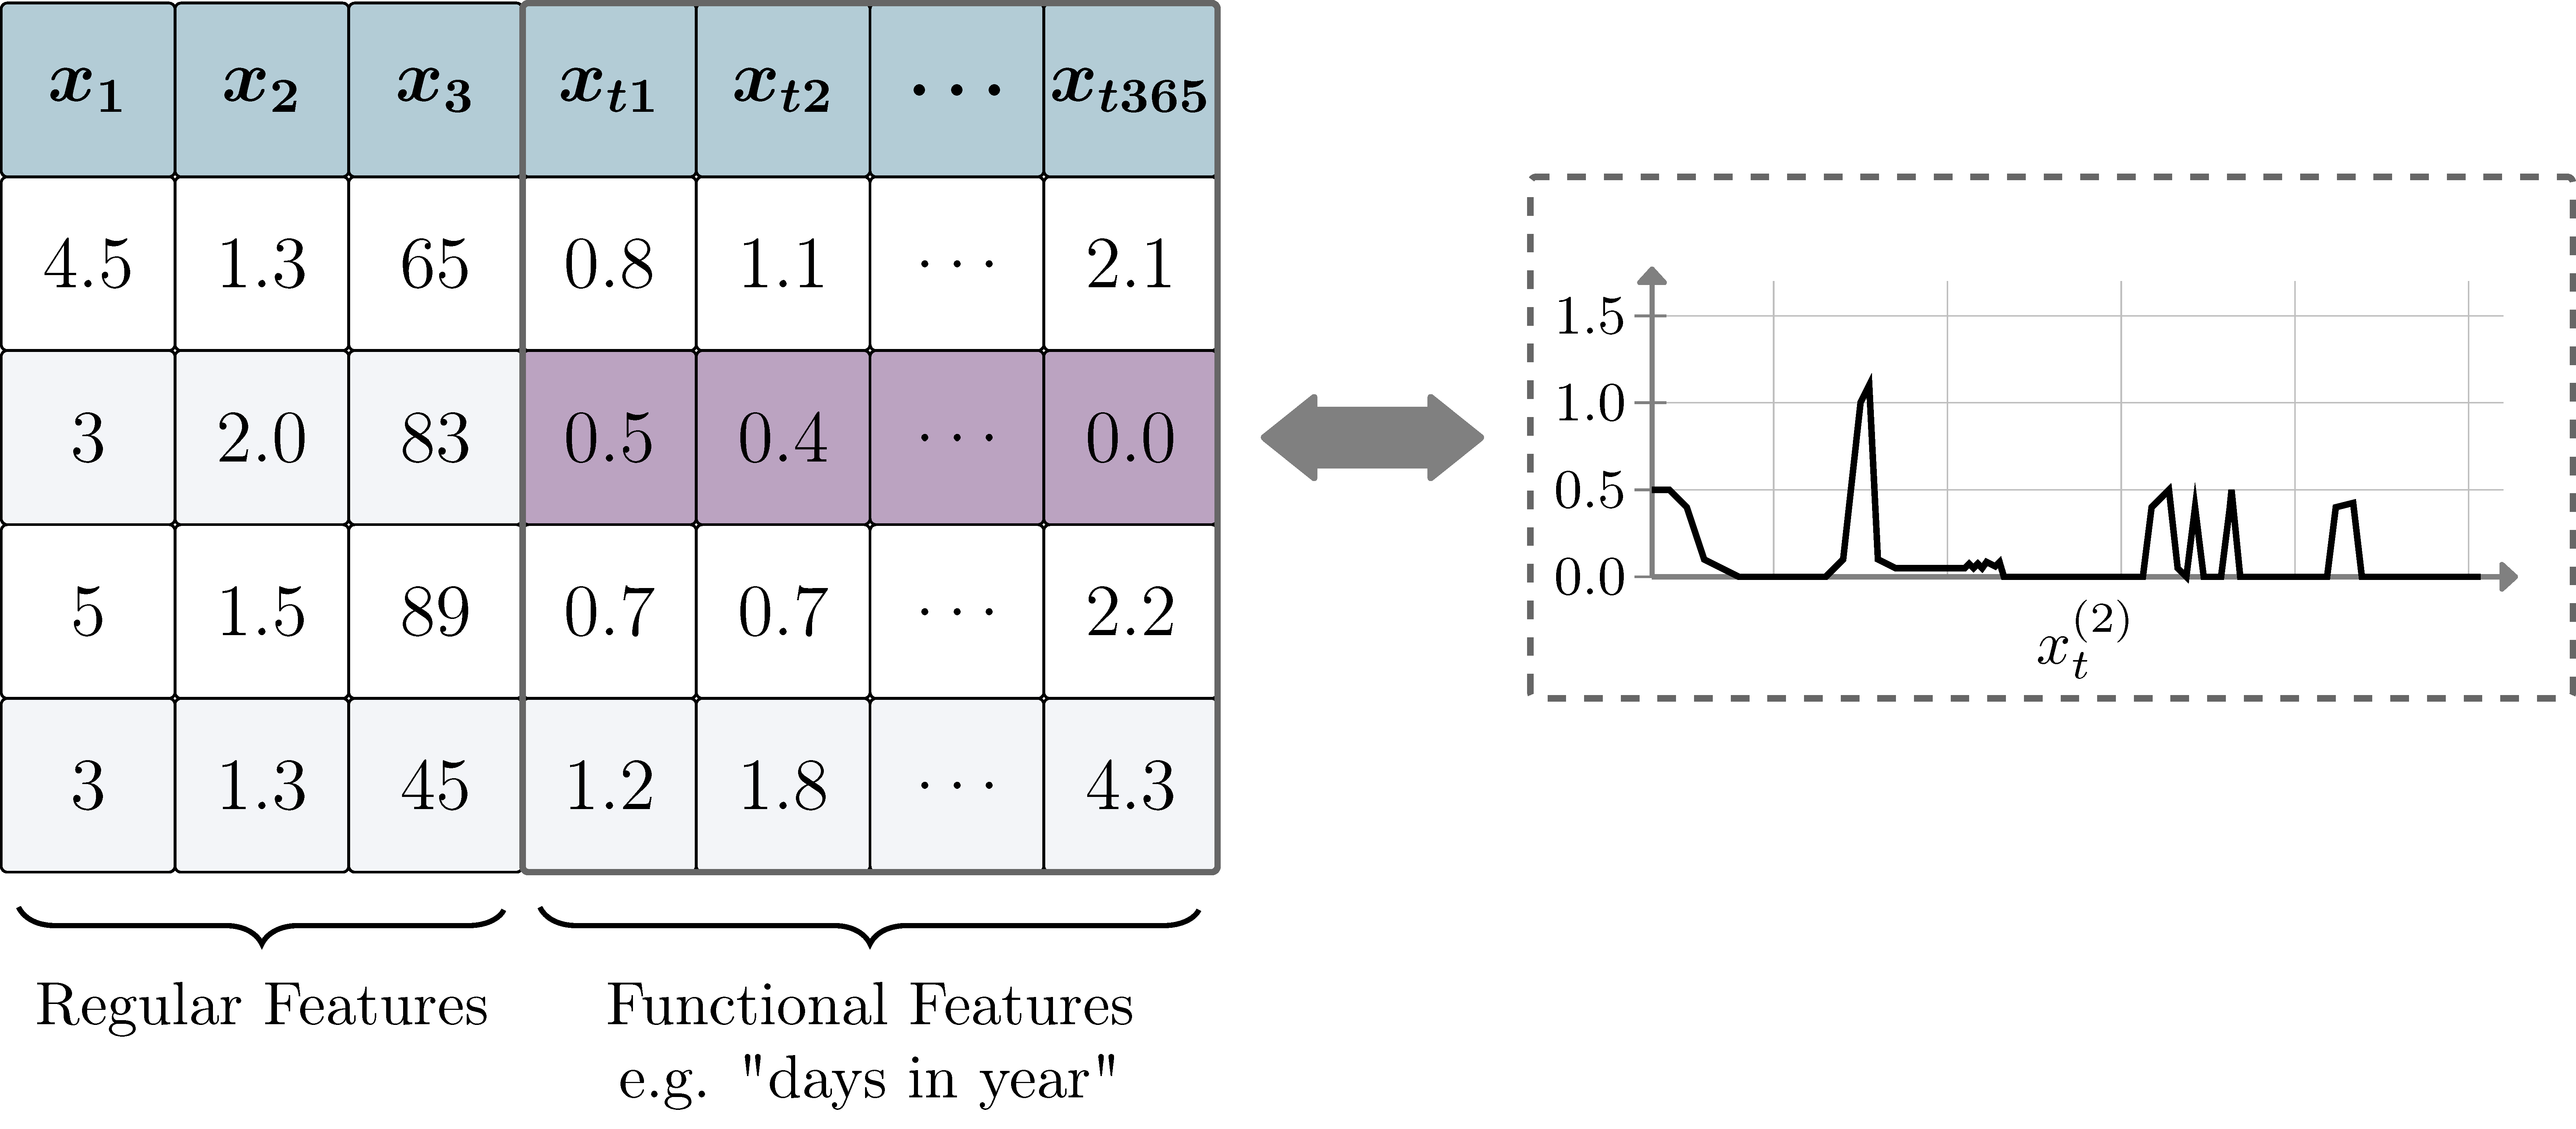
\includegraphics[width=1\textwidth,height=\textheight]{chapters/chapter9/Figures/mlr3book_figures-14.png}

}

\caption{\label{fig-functional-features}Variables x1,x2,x3 are regular
features, variables xt1,\ldots,xt365 are functional features that could
be plotted to identify important properties.}

\end{figure}

As a concrete example, consider the power consumption of kitchen
appliances in houses in the Ames dataset.

\begin{Shaded}
\begin{Highlighting}[]
\NormalTok{energy\_data }\OtherTok{=}\NormalTok{ mlr3data}\SpecialCharTok{::}\NormalTok{energy\_usage}
\end{Highlighting}
\end{Shaded}

In this dataset, each row represents one house and each feature is the
total power consumption from kitchen appliances at a given time (Bagnall
et al. 2017). The consumption is measured in two-minute intervals,
resulting in 720 features.

\begin{Shaded}
\begin{Highlighting}[]
\FunctionTok{library}\NormalTok{(ggplot2)}
\FunctionTok{ggplot}\NormalTok{(}\FunctionTok{data.frame}\NormalTok{(}\AttributeTok{y =} \FunctionTok{as.numeric}\NormalTok{(energy\_data[}\DecValTok{1}\NormalTok{, ])),}
    \FunctionTok{aes}\NormalTok{(}\AttributeTok{y =}\NormalTok{ y, }\AttributeTok{x =} \DecValTok{1}\SpecialCharTok{:}\DecValTok{720}\NormalTok{)) }\SpecialCharTok{+}
  \FunctionTok{geom\_line}\NormalTok{() }\SpecialCharTok{+} \FunctionTok{theme\_minimal}\NormalTok{() }\SpecialCharTok{+}
  \FunctionTok{labs}\NormalTok{(}\AttributeTok{x =} \StringTok{"2{-}Minute Interval"}\NormalTok{, }\AttributeTok{y =} \StringTok{"Power Consumption"}\NormalTok{)}
\end{Highlighting}
\end{Shaded}

\begin{figure}[H]

{\centering 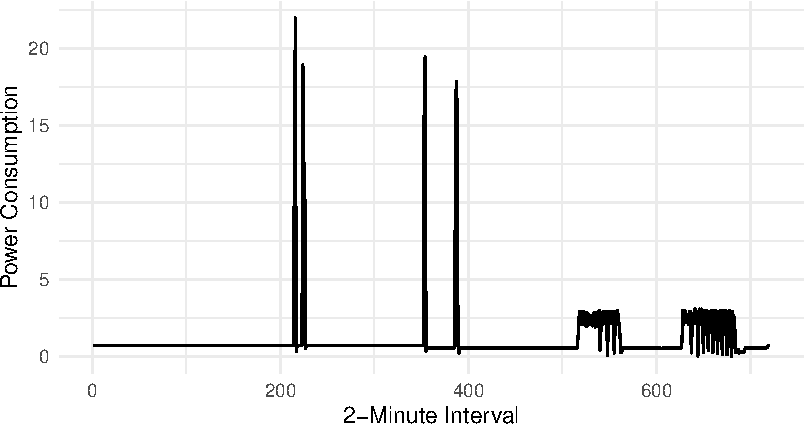
\includegraphics[width=1\textwidth,height=\textheight]{chapters/chapter9/preprocessing_files/figure-pdf/fig-energy-1.pdf}

}

\caption{\label{fig-energy}Energy consumption of one example house in a
day, recorded in two-minute intervals.}

\end{figure}

Adding these 720 features to our full dataset is a bad idea as each
individual feature does not provide meaningful information, similarly,
we cannot automate selection of the best feature subset for the same
reason. Instead, we can \emph{extract} information about the curves to
gain insights into the kitchen's overall energy usage. For example, we
could extract the maximum used wattage, overall used wattage, number of
peaks, and other similar features.

To extract features we will write our own
\href{https://mlr3pipelines.mlr-org.com/reference/PipeOp.html}{\texttt{PipeOp}}
that inherits from
\href{https://mlr3pipelines.mlr-org.com/reference/PipeOpTaskPreprocSimple.html}{\texttt{PipeOpTaskPreprocSimple}}.
To do this we add a private method called \texttt{.transform\_dt} that
hardcodes the operations in our task. In this example, we select the
functional features (which all start with ``att''), extract the mean,
minimum, maximum, and variance of the power consumption, and then remove
the functional features. To read more about building custom
\texttt{PipeOp}s, open the corresponding vignette by running
\texttt{vignette("extending",\ package\ =\ "mlr3pipelines")} in R.

\begin{Shaded}
\begin{Highlighting}[]
\NormalTok{PipeOpFuncExtract }\OtherTok{=}\NormalTok{ R6}\SpecialCharTok{::}\FunctionTok{R6Class}\NormalTok{(}\StringTok{"PipeOpFuncExtract"}\NormalTok{,}
  \AttributeTok{inherit =}\NormalTok{ mlr3pipelines}\SpecialCharTok{::}\NormalTok{PipeOpTaskPreprocSimple,}
  \AttributeTok{private =} \FunctionTok{list}\NormalTok{(}
    \AttributeTok{.transform\_dt =} \ControlFlowTok{function}\NormalTok{(dt, levels) \{}
\NormalTok{        ffeat\_names }\OtherTok{=} \FunctionTok{paste0}\NormalTok{(}\StringTok{"att"}\NormalTok{, }\DecValTok{1}\SpecialCharTok{:}\DecValTok{720}\NormalTok{)}
\NormalTok{        ffeats }\OtherTok{=}\NormalTok{ dt[, ..ffeat\_names]}
\NormalTok{        dt[, energy\_means }\SpecialCharTok{:}\ErrorTok{=} \FunctionTok{apply}\NormalTok{(ffeats, }\DecValTok{1}\NormalTok{, mean)]}
\NormalTok{        dt[, energy\_mins }\SpecialCharTok{:}\ErrorTok{=} \FunctionTok{apply}\NormalTok{(ffeats, }\DecValTok{1}\NormalTok{, min)]}
\NormalTok{        dt[, energy\_maxs }\SpecialCharTok{:}\ErrorTok{=} \FunctionTok{apply}\NormalTok{(ffeats, }\DecValTok{1}\NormalTok{, max)]}
\NormalTok{        dt[, energy\_vars }\SpecialCharTok{:}\ErrorTok{=} \FunctionTok{apply}\NormalTok{(ffeats, }\DecValTok{1}\NormalTok{, var)]}
\NormalTok{        dt[, (ffeat\_names) }\SpecialCharTok{:}\ErrorTok{=} \ConstantTok{NULL}\NormalTok{]}
\NormalTok{        dt}
\NormalTok{    \}}
\NormalTok{  )}
\NormalTok{)}
\end{Highlighting}
\end{Shaded}

Before using this in an experiment we first test that the
\texttt{PipeOp} works as expected.

\begin{Shaded}
\begin{Highlighting}[]
\NormalTok{tsk\_ames\_ext }\OtherTok{=} \FunctionTok{cbind}\NormalTok{(ames, energy\_data)}
\NormalTok{tsk\_ames\_ext }\OtherTok{=} \FunctionTok{as\_task\_regr}\NormalTok{(tsk\_ames\_ext, }\StringTok{"Sale\_Price"}\NormalTok{, }\StringTok{"ames\_ext"}\NormalTok{)}
\CommentTok{\# remove the redundant variables identified at the start of this chapter}
\NormalTok{tsk\_ames\_ext}\SpecialCharTok{$}\FunctionTok{select}\NormalTok{(}\FunctionTok{setdiff}\NormalTok{(tsk\_ames\_ext}\SpecialCharTok{$}\NormalTok{feature\_names, to\_remove))}

\NormalTok{func\_extractor }\OtherTok{=}\NormalTok{ PipeOpFuncExtract}\SpecialCharTok{$}\FunctionTok{new}\NormalTok{(}\StringTok{"energy\_extract"}\NormalTok{)}
\NormalTok{tsk\_ames\_ext }\OtherTok{=}\NormalTok{ func\_extractor}\SpecialCharTok{$}\FunctionTok{train}\NormalTok{(}\FunctionTok{list}\NormalTok{(tsk\_ames\_ext))[[}\DecValTok{1}\NormalTok{]]}
\NormalTok{tsk\_ames\_ext}\SpecialCharTok{$}\FunctionTok{data}\NormalTok{(}\DecValTok{1}\NormalTok{,}
  \FunctionTok{c}\NormalTok{(}\StringTok{"energy\_means"}\NormalTok{, }\StringTok{"energy\_mins"}\NormalTok{, }\StringTok{"energy\_maxs"}\NormalTok{, }\StringTok{"energy\_vars"}\NormalTok{))}
\end{Highlighting}
\end{Shaded}

\begin{verbatim}
   energy_means energy_mins energy_maxs energy_vars
1:        1.062     0.01427       21.98       3.708
\end{verbatim}

These outputs look sensible compared to Figure~\ref{fig-energy} so we
can now run our final benchmark experiment using feature extraction. We
do not need to add the \texttt{PipeOp} to each learner as we can apply
it once (as above) before any model training by applying it to all
available data.

\begin{Shaded}
\begin{Highlighting}[]
\NormalTok{learners }\OtherTok{=} \FunctionTok{list}\NormalTok{(lrn\_baseline, }\FunctionTok{lrn}\NormalTok{(}\StringTok{"regr.rpart"}\NormalTok{), glrn\_xgb\_impact,}
\NormalTok{    glrn\_rf\_impute\_oor, glrn\_lm\_robust, glrn\_log\_lm\_robust)}

\NormalTok{bmr\_final }\OtherTok{=} \FunctionTok{benchmark}\NormalTok{(}\FunctionTok{benchmark\_grid}\NormalTok{(}\FunctionTok{c}\NormalTok{(tsk\_ames\_ext, tsk\_ames), learners,}
\NormalTok{  rsmp\_cv3))}

\NormalTok{perf }\OtherTok{=}\NormalTok{ bmr\_final}\SpecialCharTok{$}\FunctionTok{aggregate}\NormalTok{(}\AttributeTok{measure =}\NormalTok{ msr\_mae)}
\NormalTok{perf[}\FunctionTok{order}\NormalTok{(learner\_id, task\_id), .(task\_id, learner\_id, regr.mae)]}
\end{Highlighting}
\end{Shaded}

\begin{verbatim}
     task_id         learner_id regr.mae
 1:     ames           Baseline    56056
 2: ames_ext           Baseline    56056
 3:     ames         RF_imp_OOR    16433
 4: ames_ext         RF_imp_OOR    14317
 5:     ames     XGB_enc_impact    16068
 6: ames_ext     XGB_enc_impact    14400
 7:     ames          lm_robust    16291
 8: ames_ext          lm_robust    15093
 9:     ames lm_robust_logtrafo    15555
10: ames_ext lm_robust_logtrafo    13905
11:     ames         regr.rpart    27371
12: ames_ext         regr.rpart    27111
\end{verbatim}

The final results indicate that adding these extracted features improved
the performance of all models (except the featureless baseline).

In this example, we could have just applied the transformations to the
dataset directly and not used a \texttt{PipeOp}. However, the advantage
of using the \texttt{PipeOp} is that we could have chained it to a
subset of learners to prevent a blow-up of experiments in the benchmark
experiment.

\hypertarget{conclusion-7}{%
\section{Conclusion}\label{conclusion-7}}

In this chapter, we built on everything learned in
Chapter~\ref{sec-pipelines} and Chapter~\ref{sec-pipelines-nonseq} to
look at concrete usage of pipelines for data preprocessing. We focused
primarily on feature engineering, which can make use of
\href{https://mlr3pipelines.mlr-org.com}{\texttt{mlr3pipelines}}\index{\texttt{mlr3pipelines}}
to automate preprocessing as much as possible while still ensuring user
control. We looked at factor encoding for categorical variables,
imputing missing data, transforming variables, and feature extraction.
Preprocessing is almost always required in machine learning experiments,
and applying the \texttt{ppl("robustify")} will help in many cases to
simplify this process by applying the most common preprocessing steps,
we will see this in use in Chapter~\ref{sec-large-benchmarking}.

We have not introduced any new classes in this chapter, so instead
Table~\ref{tbl-prepro-api} lists the
\href{https://mlr3pipelines.mlr-org.com/reference/PipeOp.html}{\texttt{PipeOp}}s
and
\href{https://mlr3pipelines.mlr-org.com/reference/Graph.html}{\texttt{Graph}}s
we discussed.

\hypertarget{tbl-prepro-api}{}
\begin{longtable}[]{@{}
  >{\raggedright\arraybackslash}p{(\columnwidth - 2\tabcolsep) * \real{0.4000}}
  >{\raggedright\arraybackslash}p{(\columnwidth - 2\tabcolsep) * \real{0.6000}}@{}}
\caption{\label{tbl-prepro-api}\texttt{PipeOp}s and \texttt{Graph}s
discussed in this chapter.}\tabularnewline
\toprule\noalign{}
\begin{minipage}[b]{\linewidth}\raggedright
PipeOp/Graph
\end{minipage} & \begin{minipage}[b]{\linewidth}\raggedright
Description
\end{minipage} \\
\midrule\noalign{}
\endfirsthead
\toprule\noalign{}
\begin{minipage}[b]{\linewidth}\raggedright
PipeOp/Graph
\end{minipage} & \begin{minipage}[b]{\linewidth}\raggedright
Description
\end{minipage} \\
\midrule\noalign{}
\endhead
\bottomrule\noalign{}
\endlastfoot
\href{https://mlr3pipelines.mlr-org.com/reference/mlr_pipeops_removeconstants.html}{\texttt{PipeOpRemoveConstants}}
& Remove variables consisting of one value \\
\href{https://mlr3pipelines.mlr-org.com/reference/mlr_pipeops_collapsefactors.html}{\texttt{PipeOpCollapseFactors}}
& Combine rare factor levels \\
\href{https://mlr3pipelines.mlr-org.com/reference/mlr_pipeops_encodeimpact.html}{\texttt{PipeOpEncodeImpact}}
& Impact encoding \\
\href{https://mlr3pipelines.mlr-org.com/reference/mlr_pipeops_encode.html}{\texttt{PipeOpEncode}}
& Other factor encoding methods \\
\href{https://mlr3pipelines.mlr-org.com/reference/mlr_pipeops_missind.html}{\texttt{PipeOpMissInd}}
& Add an indicator column to track missing data \\
\href{https://mlr3pipelines.mlr-org.com/reference/mlr_pipeops_imputehist.html}{\texttt{PipeOpImputeHist}}
& Impute missing data by sampling from a histogram \\
\href{https://mlr3pipelines.mlr-org.com/reference/mlr_pipeops_imputeoor.html}{\texttt{PipeOpImputeOOR}}
& Impute missing data with out-of-range values \\
\href{https://mlr3pipelines.mlr-org.com/reference/mlr_graphs_robustify.html}{\texttt{pipeline\_robustify}}
& Graph with common imputation and encoding methods \\
\href{https://mlr3pipelines.mlr-org.com/reference/mlr_graphs_targettrafo.html}{\texttt{pipeline\_targettrafo}}
& Graph to transform target during training and invert transformation
during prediction \\
\end{longtable}

\hypertarget{exercises-7}{%
\section{Exercises}\label{exercises-7}}

We will consider a prediction problem similar to the one from this
chapter, but using the King County Housing regression data instead
(available with \texttt{tsk("kc\_housing")}). To evaluate the models, we
again use 10-fold CV, mean absolute error and
\texttt{lrn("regr.glmnet")}. For now we will ignore the \texttt{date}
column and simply remove it:

\begin{Shaded}
\begin{Highlighting}[]
\FunctionTok{library}\NormalTok{(}\StringTok{"mlr3data"}\NormalTok{)}
\NormalTok{kc\_housing }\OtherTok{=} \FunctionTok{tsk}\NormalTok{(}\StringTok{"kc\_housing"}\NormalTok{)}
\NormalTok{kc\_housing}\SpecialCharTok{$}\FunctionTok{select}\NormalTok{(}\FunctionTok{setdiff}\NormalTok{(kc\_housing}\SpecialCharTok{$}\NormalTok{feature\_names, }\StringTok{"date"}\NormalTok{))}
\end{Highlighting}
\end{Shaded}

\begin{enumerate}
\def\labelenumi{\arabic{enumi}.}
\tightlist
\item
  Have a look at the features, are there any features which might be
  problematic? If so, change or remove them. Check the dataset and
  learner properties to understand which preprocessing steps you need to
  do.
\item
  Build a suitable pipeline that allows \texttt{glmnet} to be trained on
  the dataset. Construct a new \texttt{glmnet} model with
  \texttt{ppl("robustify")}. Compare the two pipelines in a benchmark
  experiment.
\item
  Now consider the \texttt{date} feature: How can you extract
  information from this feature in a way that \texttt{glmnet} can use?
  Does this improve the performance of your pipeline? Finally, consider
  the spatial nature of the dataset. Can you extract an additional
  feature from the lat / long coordinates? (Hint: Downtown Seattle has
  lat/long coordinates \texttt{47.605}/\texttt{122.334}).
\end{enumerate}
